%\documentclass{article}
%\usepackage{tikz}
%\usepackage{SIunits}
%\begin{document}

\begin{figure}[tb]
	\centering
	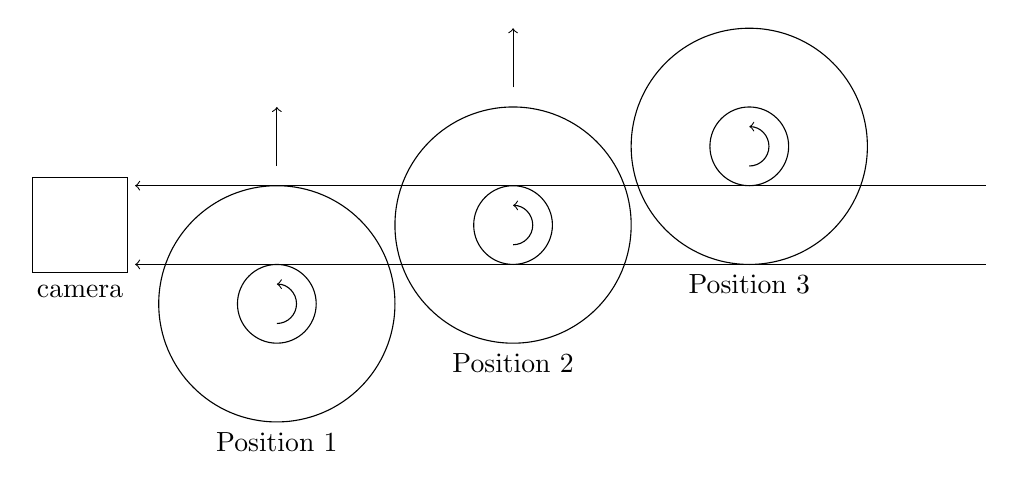
\begin{tikzpicture}
		%drawing grid
%		\draw[color=gray] (0,0) grid (10,1);
		%camera
			\draw (-.1,-.1) rectangle (1.1,1.1);
			\draw (.5,-.35) node {camera};
		% sample positions
			\foreach \x in {1,2,3}{
				\draw (3*\x,\x-1.5) circle (.5) circle (1.5);			
				\draw[->] (3*\x,\x-1.75) arc (-90:90:.25);
				\draw (3*\x,-3.25+\x)node {Position \x};
				}
		% movement		
			\foreach \x in {1,2}{				
			    \draw[->]  (3*\x,0.25+\x) -- (3*\x,1+\x);
		% beam
				\draw[<-] (1.2,\x-1) -- (12,\x-1);
				}
	\end{tikzpicture}
	\caption{Covering the FOV -- three scans $\rightarrow$ sample has to move, explain that we still only do \unit{180}{\degree} scans!}
	\label{fig:covering-three scans}
\end{figure}

\begin{figure}[tb]
	\centering
	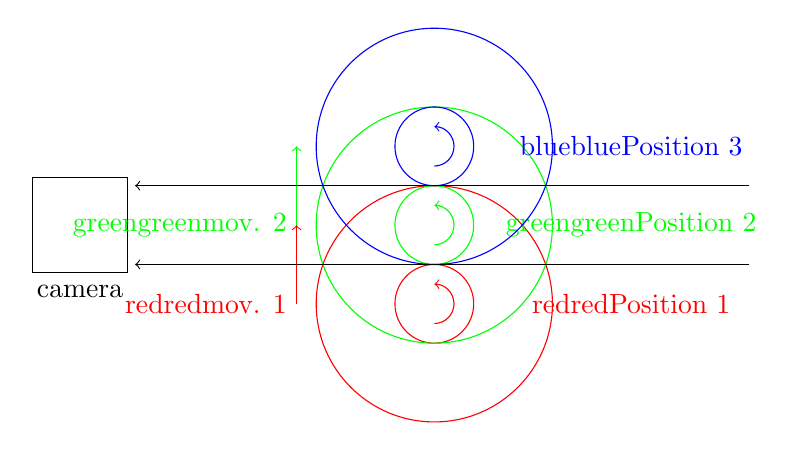
\begin{tikzpicture}
		%camera
			\draw (-.1,-.1) rectangle (1.1,1.1);
			\draw (.5,-.35) node {camera};
		% sample positions
			\foreach \x/\color in {1/red,2/green,3/blue}{
				\draw[color=\color]    (5,\x-1.5) circle (.5) circle (1.5);			
				\draw[color=\color,->] (5,\x-1.75) arc (-90:90:.25);
				\draw[color=\color]    (7.5,\x-1.5)node {Position \x};
				}
		% movement		
			\foreach \x/\e/\color in {1/3.25/red,2/3.25/green}{				
			    \draw[color=\color,->] (\e,-1.5+\x) node [left] {mov. \x} -- (\e,-.5+\x);
			    }
			 \foreach \x in {1,2}{				
		% beam
				\draw[<-] (1.2,\x-1) -- (9,\x-1);
				}
	\end{tikzpicture}
	\caption{Covering the FOV -- three scans $\rightarrow$ sample has to move, explain that we still only do \unit{180}{\degree} scans!}
	\label{fig:covering-three scans}
\end{figure}

%\end{document}